%; whizzy section -pdf xpdf -latex ./whizzypdfptex.sh
% latex beamer presentation.
% platex, latex-beamer でコンパイルすることを想定。

%     Tokyo Debian Meeting resources
%     Copyright (C) 2007 Junichi Uekawa

%     This program is free software; you can redistribute it and/or modify
%     it under the terms of the GNU General Public License as published by
%     the Free Software Foundation; either version 2 of the License, or
%     (at your option) any later version.

%     This program is distributed in the hope that it will be useful,
%     but WITHOUT ANY WARRANTY; without even the implied warranty of
%     MERCHANTABILITY or FITNESS FOR A PARTICULAR PURPOSE.  See the
%     GNU General Public License for more details.

%     You should have received a copy of the GNU General Public License
%     along with this program; if not, write to the Free Software
%     Foundation, Inc., 51 Franklin St, Fifth Floor, Boston, MA  02110-1301 USA

% 実行順番
% sudo  ~/bin/usb-macbook-ir.c &
% real presentation (shell-command (concat "DISPLAY=:0.1 xpdf -fullscreen " (replace-regexp-in-string "tex$" "pdf"(buffer-file-name)) "&"))
% DISPLAY=:0.1 xpdf -fullscreen

\documentclass[cjk,dvipdfmx,12pt]{beamer}
\usetheme{Tokyo}
\usepackage{ulem}
\usepackage{tabularx}

\usepackage{fancybox}
\usepackage{fancyvrb}
\usepackage{float}
\usepackage[english]{babel}
% commandline環境を定義。画面入出力についてはcommandline環境
% で表記する
\newenvironment{commandline}%
{\VerbatimEnvironment
  \begin{Sbox}\begin{minipage}{0.9\hsize}\begin{fontsize}{7.3}{7.3} \begin{BVerbatim}}%
{\end{BVerbatim}\end{fontsize}\end{minipage}\end{Sbox}
  \setlength{\fboxsep}{8pt}
% start on a new paragraph

\vspace{6pt}% skip before
\fcolorbox{dancerdarkblue}{dancerlightblue}{\TheSbox}

\vspace{6pt}% skip after
}
%end of commandline

\definecolor{dancerdarkblue}{rgb}{0,0.08,0.45}
\definecolor{dancernormalblue}{rgb}{0.8,0.9,0.95}
\definecolor{dancerlightblue}{rgb}{0.8,0.95,1}


%  preview (shell-command (concat "evince " (replace-regexp-in-string "tex$" "pdf"(buffer-file-name)) "&"))
%  presentation (shell-command (concat "xpdf -fullscreen " (replace-regexp-in-string "tex$" "pdf"(buffer-file-name)) "&"))

%http://www.naney.org/diki/dk/hyperref.html
%日本語EUC系環境の時
\AtBeginDvi{\special{pdf:tounicode EUC-UCS2}}
%シフトJIS系環境の時
%\AtBeginDvi{\special{pdf:tounicode 90ms-RKSJ-UCS2}}

\title{東京エリア Debian 勉強会}
\subtitle{資料}
\author{上川 純一 dancer@debian.org\\IRC nick: dancerj}
\date{2007年11月17日}
\logo{
\includegraphics[width=8cm]{image200607/openlogo-light.eps}}


% 間のタイトルページ用
\newcommand{\emtext}[1]{
\begin{frame}{}

\begin{minipage}{0.55\hsize}
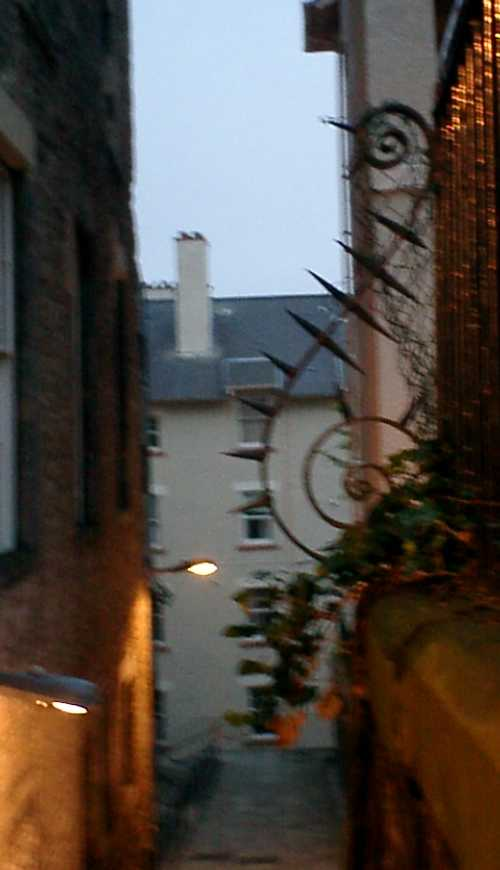
\includegraphics[width=1\hsize]{image200707/gurutitle.jpg}
\end{minipage}
\begin{minipage}{0.39\hsize}
 {\Huge #1
 }
\end{minipage}
\end{frame}
}

% 三択問題用
\newcounter{santakucounter}
\newcommand{\santaku}[5]{%
\addtocounter{santakucounter}{1}
\frame{\frametitle{問題\arabic{santakucounter}. #1}
%問題\arabic{santakucounter}. #1
\begin{minipage}[t]{0.8\hsize}
 \begin{itemize}
 \item
      \begin{minipage}{0.2\hsize}
      
\includegraphics[width=0.9\hsize]{image200703/janken-A.png}\end{minipage}
       \begin{minipage}{0.6\hsize}
       A #2\end{minipage}\\
 \item
      \begin{minipage}{0.2\hsize}
      
\includegraphics[width=0.9\hsize]{image200703/janken-B.png}\end{minipage}
       \begin{minipage}{0.6\hsize}
       B #3\end{minipage}\\
 \item
      \begin{minipage}{0.2\hsize}
      
\includegraphics[width=0.9\hsize]{image200703/janken-C.png}\end{minipage}
       \begin{minipage}{0.6\hsize}
       C #4\end{minipage}\\
 \end{itemize}
\end{minipage}
}
\frame{\frametitle{問題\arabic{santakucounter}. #1}
%問題\arabic{santakucounter}. #1
\begin{minipage}[t]{0.8\hsize}
\begin{itemize}
 \item
      \begin{minipage}{0.2\hsize}
      
\includegraphics[width=0.9\hsize]{image200703/janken-A.png}\end{minipage}
       \begin{minipage}{0.6\hsize}
       A #2\end{minipage}\\
 \item
      \begin{minipage}{0.2\hsize}
      
\includegraphics[width=0.9\hsize]{image200703/janken-B.png}\end{minipage}
       \begin{minipage}{0.6\hsize}
       B #3\end{minipage}\\
 \item
      \begin{minipage}{0.2\hsize}
      
\includegraphics[width=0.9\hsize]{image200703/janken-C.png}\end{minipage}
       \begin{minipage}{0.6\hsize}
       C #4\end{minipage}\\
\end{itemize}
\end{minipage}
\begin{minipage}[t]{0.15\hsize}
答えは:

\vspace{1cm}

  {\huge \hspace{1cm}#5}
  \hspace{-6cm}\includegraphics[width=4cm]{image200703/janken-#5.png}
 \end{minipage}}
}

\begin{document}
\frame{\titlepage{}}

\section{Intro}

\begin{frame}
 \frametitle{Agenda}
\begin{minipage}[t]{0.45\hsize}
  \begin{itemize}
  \item 注意事項
	\begin{itemize}
	 \item 飲食禁止
	 \item 政治/宗教/営利活動禁止
	\end{itemize}
  \item quiz
  \item 最近のDebian関連のイベント
	\begin{itemize}
	 \item 前回
	 \item OSC Tokyo/Fall
	 \item KOF
	 \item Biella 宴会
	\end{itemize}
 \end{itemize}
\end{minipage}
\begin{minipage}[t]{0.45\hsize}
 \begin{itemize}
  \item bluetooth
  \item livehelper
  \item tomoyo kernel module
  \item KOF
  \item OSC Tokyo/Fall
  \item 今後の計画
 \end{itemize}
\end{minipage}
\end{frame}

\section{最近}

\begin{frame}
 \frametitle{前々回のAgenda}
\begin{minipage}[t]{0.45\hsize}
  \begin{itemize}
  \item 注意事項
	\begin{itemize}
	 \item 飲食禁止
	 \item 政治/宗教/営利活動禁止
	\end{itemize}
  \item quiz
  \item 最近のDebian関連のイベント
	\begin{itemize}
	 \item 前回
	 \item コミケ
	 \item 1st Debian JP BSP
	\end{itemize}
 \end{itemize}
\end{minipage}
\begin{minipage}[t]{0.45\hsize}
 \begin{itemize}
  \item Exim
  \item MTA/MUA,ネットワークプロトコル
 \end{itemize}
\end{minipage}
\end{frame}



\section{DWN quiz}
\begin{frame}{Debian 常識クイズ}

Debian の常識、もちろん知ってますよね?
知らないなんて恥ずかしくて、知らないとは言えないあんなことやこんなこと、
みんなで確認してみましょう。

今回の出題範囲は、\url{http://lists.debian.org/debian-devel-announce/} にある最近の
アナウンス文書です。

\end{frame}

\subsection{問題}

 \santaku
 {10/4 にアナウンスがあった alioth のサービスに追加されたものは?}
 {VSSサポート}
 {darcsサポート}
 {p4サポート}
 {B}

 \santaku
 {DebianGisチームは何をするチームか?}
 {Gisのパッケージのメンテナンス}
 {DebianをGisでのっとるプロジェクト}
 {人間関係をギスギスしてみる}
 {A}

 \santaku
 {testing security のメールの仕組みで何がかわったか}
 {unstable から testing へのマイグレーションでセキュリティーバグが修正さ
 れてもアナウンスされるようにした}
 {昨年度 Debian testing security team がCVEを5500も処理したことが自慢できるようになった}
 {SMTPプロトコルのハンドシェークが変わった}
 {A}


 \santaku
 {Debconf8 の日程は}
 {5月1日から5月10日}
 {8月2日から8月17日}
 {12月24日から1月1日}
 {B}

 \santaku
 {http://security-tracker.debian.net/tracker/ で何が見れるか}
 {手元のマシンが脆弱化どうかの試験}
 {セキュリティーについての入門}
 {セキュリティーバグの現在の状態}
 {C}

 \santaku
 {Debian System Administrator として新しく任命されたのは誰か}
 {Sven Luther}
 {Phil Hands}
 {Peter Palfrader}
 {C}

 \santaku
 {ries.debian.org (ftp-master) はどれくらい停止していたか}
 {11月5日から11月12日}
 {11月5日から11月30日}
 {11月1日から11月5日}
 {A}


\section{最近の話題}

% のちほど報告、かな。
\emtext{OSC Tokyo/Fall}
\emtext{KOF}
\emtext{Biella 宴会}

\begin{frame}{Biella Colemanを囲む会}
\begin{itemize}
 \item  参加者
 \begin{itemize}
 \item New York University の Biella Coleman と Aram Sinnreich
 \item Creative Commons の Asheesh
 \item Debian JP の knok、mhatta、dancerj
 \end{itemize}
 \item 会場: 銀座の「がんこ」
 \item 開催場所: 11月14日

\end{itemize}

DebianのNMプロセスについて、Debianはオープンだがエリート主義か、ポピュリ
ストかどうかということで激論をかわしました。
\end{frame}


\section{事前課題紹介}
\emtext{事前課題の紹介}
% pre work home work

\begin{frame}{事前課題問題}
「Debian の Live CD ってこんなふうに使ってます」もしくは「ノートPCやデスクトップPCではなく、サーバ機器での Debian に期待するものって何?」というタイトルで200-800文字程度の文章を書いてください。
\end{frame}

% (query-replace "\\subsection" "\\end{frame}\\begin{frame}")
% (query-replace "\\subsubsection" "\\textbf")


\begin{frame}{前田 耕平}

\textbf{「ノートPCやデスクトップPCではなく、サーバ機器での Debian に期待するものって何?」}
完全な最小構成のインストーラですね。Debianでもやっぱり最小構成でインストールしても無駄なパッケージが多いので、サーバを構築するときは必ず最小構成でインストール後にさらにそこから引っこ抜いています。
Sargeに比べたらEtchは結構良くなったと思いますけど、まだ足りない、もとい多いですね。
RHELとかSUSEなんて多すぎて論外ですけど。

\textbf{「Debian の Live CD ってこんなふうに使ってます」}
DebianのLive CDは正直使ったことはありません。Live CDは、重いですけどKNOPPIX使ってます。
USB-KNOPPIXなんかも使っていたりしますが、CD-ROMよりは軽いです。
KNOPPIXがもともとDebianベースだと言っても、APT使わなければ意味ないですね。
使い方としては、やっぱりIAサーバのメンテナンスや、期間が短いテストを行うときに使っています。

\end{frame}\begin{frame}{satoken}

\textbf{ノートPCやデスクトップPCではなく、
サーバ機器での Debian に期待するものって何?}

\begin{description}
 \item[安定性]
  多少古くても安定していて欲しい....と言う点でDebianは良さそう
  でも、本当にそうだろうか? そうだと思いたいんだけど...

 \item[構築容易性]
  Installしてから動かす迄に必要な設定が少なくて済む。
  依存性を考慮して必要な物はついでに入れてくれるし。
  他のディストリビューションでは設定作業量が何かと多い気が...

 \item[パッケージ管理]
  aptに感動。
  ところで、apt-cacherの話は?ありますでしょうか?期待してます。
 (apt-proxyが落ちやすいので)
\end{description}

\end{frame}\begin{frame}{satoken}

期待したいんだけど期待できない点

\begin{description}
 \item[最新ハードウェア対応]
  Ubuntuからのフィードバックで加速されるかなぁ?

 \item[有償ソフト対応]
  「Debianでも動く」と言ってくれるソフトがとても少ない。
  DELLがUbuntu搭載PCの日本語版を出してくれれば.....
\end{description}


 と言う感じで、Ubuntuが流行ればDebianにも良い影響が
波及してくるのでは?と期待してます。


\end{frame}\begin{frame}{jun araki}
\textbf{サーバ機器での Debian に期待するものって何?}

サーバ機器の場合、まず OS としての安定性(可用性)とセキュリティを期待します。
それぞれ Debian について考えてみますと、以下のような点が強みとして挙げられると思います。

	    \begin{itemize}
	     \item  安定性(可用性)
		    \begin{itemize}
		     \item  sid, testing, stable といったリリースサイクルによる厳格なテストと品質管理
		     \item  高可用性を実現する為のパッケージ(Idirectord
			    \footnote{ldirectord, \url{http://www.vergenet.net/linux/ldirectord/}},
			    Ultra Monkey
			    \footnote{Ultra Monkey, http://ultramonkey.jp/} など)が提供されていること
		    \end{itemize}

	     \item  セキュリティ
	     \begin{itemize}
	      \item  ML によるセキュリティ関連のアナウンス
	      \item  上記のテストや品質管理をベースとしたセキュリティアップデート
	     \end{itemize}
	    \end{itemize}

\end{frame}\begin{frame}{jun araki}

 これら以外には、サーバ管理やインストールの容易性を期待します。


 サーバ台数が増えてくると、ハードウェアの故障件数も増えてきますので、
 OS の比較的頻繁な入れ替えやバージョンの異なる OS を(一時的に)共存
 させた状態での運用といったことも想定されます。

 それに対して、Debian の場合サーバ管理については、

	    \begin{itemize}
	     \item  FHS(File Hierarchy Standard)準拠による透過性
	     \item  自動化ツール群の豊富さ
	    \end{itemize}

といったところが特徴かと思います。\footnote{"The Debian System --- その概念と技法"}
ツールの方はまだそれほど使いこなしてはないのでこれから試してみます。

\end{frame}\begin{frame}{jun araki}

インストールについては、これもまだ使ったことがないのですが、 preseed
による自動インストールというのがあります。ただ、既存のパーティションを
利用できない(パーティションを再作成するか空き領域を利用するかしかない)
といった制限があるようです。\footnote{ "Debian GNU/Linux インストールガイド B.1.2. 制限",
\url{http://www.debian.org/releases/stable/mipsel/apbs01.html.ja\#preseed-limitations}}

\end{frame}\begin{frame}{山本 琢}

\textbf{Debianにサーバとして期待すること。}

\begin{description}
 \item[シェルスクリプトを書かずに管理できるようにしたい]
	    今のLinuxは敷居が高いと思う
 \item[kickstart(自動OSインストール)のサポート]
	    一度に複数の同一形式PCにインストールしたい
 \item[各種ログ出力のカスタマイズが容易に出来ること ]
	    (syslog-ngのカスタマイズ)
	    ログ出力設定が難しい
 \item[TOMOYO(若しくはAppArmor)のサポート]
	    セキュリティー管理をSELinux以外の選択肢が欲しい
 \item[DBレプリケーション設定のGUI化 ]
	    (dpkg-reconfigureのようなもの)
	    Debianの管理ツールで容易に設定出来ると嬉しい
\end{description}

\end{frame}\begin{frame}{Hajime Fukuda}

\textbf{「ノートPCやデスクトップPCではなく、サーバ機器での Debian に期待するものって何?」}

僕がサーバでDebianを使っている理由として、最小構成でのインストールが容易で、またaptをつかえば簡単に新しいパッケージを入れられるということがある。サーバではなるべく余計なものを入れないということが基本であるので、Debianのこの性格はサーバにとても適していると思う。
また、Debianでは、サーバの設定は基本的にviなどで設定ファイルを手で編集して適用する。他のディストリビューションではなんだかGUI設定ツールがたくさんついているが、サーバにXは不要だし、こみいった設定などはやはりファイルを直接編集した方がやりやすいと思う。僕はこういったところもDebianをサーバに選ぶポイントにしている。

\end{frame}\begin{frame}{小林 `nori1' 儀匡}

\textbf{「Debian の Live CD ってこんなふうに使ってます」}

Live CDと言えるのか微妙ですが、インストーラCDをレスキュー用に使っています。

また、ぼく自身は使ったことはないのですが、何年か前に、GNU/Linux環境に
慣れていないWindowsユーザが統計言語 GNU R など研究者に有用なソフトウェ
アを手軽に使用できる方法としてKnoppixがよく紹介されていた覚えがありま
す (今でもそうかもしれませんが、今だとCygwin上でX環境を構築するのも楽
でしょうし、そもそもCygwinさえ通さずにWindowsネイティブアプリケーショ
ンとして使えるFLOSSソフトウェアも増えているので、前ほどは重要性は減っ
ているのではないかと思います)。インストールさえ敷居が高い (手を出しに
くい)、というユーザはいるはずなので、ライブ CD は重要だと思います。

\end{frame}\begin{frame}{小林 `nori1' 儀匡}
\textbf{「ノートPCやデスクトップPCではなく、サーバ機器での Debian に期待するものって何?」}

最小構成でインストールでき、必要なものは追加で簡単にインストールできる
こと、でしょうね。その意味でDebianは間違いなく他のディストリビューショ
ンに勝っていると思いますから、今後もその路線は維持していただきたいです。
また、ネットワークインストールによって複数のマシンに同じような環境を簡
単にセットアップできることも重要だと思いますが、ぼくは企業のような大規
模な組織でのシステム管理経験はないので単なる推測に過ぎません。


\end{frame}\begin{frame}[containsverbatim]{Hideki Yamane}

\textbf{「ノートPC やデスクトップPC ではなく、サーバ機器でのDebian に期待するものって何?」}
 もっと簡単なセットアップが出来るといいですよね。
 Windows Server 2003 の様に「○×サーバ機能」を選ぶと、ウィザードでサクッ
と入ってしまうとか。

\begin{commandline}
 ------------------------------------------------
 |  導入したいサーバ機能を選んでください
 |
 |   - LAMPサーバを纏めて導入
 |
 |   - web サーバ (apache, lighttpd)
 |   - ファイルサーバ (Samba, NFS)
 |   - DNS サーバ (bind)
 |   - DHCP サーバ (dhcp3)
 |   - LDAP サーバ (openldap)
 |   - Radius サーバ (xxx)
 |   - NTP サーバ (ntpd)
 ------------------------------------------------
\end{commandline}

 みたいな感じでさくさくできるの。

\end{frame}\begin{frame}{Hideki Yamane}

\textbf{「Debian のLive CD ってこんなふうに使ってます」}
 live-helper 使って遊んでるだけですね。もう少し楽になるように要望を出していくつもりです。

\end{frame}\begin{frame}{hiro}

\textbf{Debian の Live CD ってこんなふうに使ってます}

Debianと直接の関係はありませんが、先日gOSを使ってみました。

\textbf{ノートPCやデスクトップPCではなく、サーバ機器での Debian に期待
するものって何?}
安定性と長期のサポート。以前Fedora Coreを使用していた際、パッケー
ジのアップデートをしただけでSambaのメジャーバージョンが上がって
しまい、焦ったことがあります。またサポート期間が短いと頻繁に新し
いものへ移行しなければならず、止めづらいサーバへの導入は苦しいも
のがあります。

\end{frame}\begin{frame}{山本 浩之}

\textbf{「Debian の Live CD ってこんなふうに使ってます」}

使っていません(わら
KNOPPIX ならちょこっと使っています。
主にハードディスクエラーが出たときの fsck で使っております。
あと、パーティションを切るときに使いました。

これでは課題にならないので、こんな Debian Live CD があったらいいな、を書
きます。
CD から HDD のメンテナンスするときは、基本的に、HDD のパーティションをど
こかにマウントし、そのマウントしたディレクトリに chroot した後、HDD 内の
コマンドを使うのが一般的ですよね。
そこで、ディスクエラーなどで HDD の dpkg コマンドや apt コマンドなどの基
本的なコマンドが壊れても修復できるような、メンテナンス専用 Live CD があ
るといいです。
具体的には CD 内に存在する apt コマンドとかで HDD のパーティションに直接
パッケージ (例えば dpkg パッケージとか) がインストールできる、そんな CD
があると嬉しいです。

\end{frame}\begin{frame}{山本 浩之}

\textbf{「ノートPCやデスクトップPCではなく、サーバ機器での Debian に期待するも
のって何?」}

サーバ機器は使ってないので、あまり具体的にイメージできないのですが、一般
的には新しいパッケージより安定したパッケージを採用ってことになりますかね?
あと、24 時間稼働させるとなると、消費電力と熱のコントロールも必要になり
ますかね?
処理速度重視より、安定にエラー無く稼働することが重視されると思います。

ついでに、oldstable のセキュリティサポート期間が、現在、次の stable がリ
リースされて約一年ってことになっています。
今のところ、stable リリースのサイクルが約一年半に一度が良かろう、と言わ
れているそうですが、この残り半年間のため、一つ飛ばしの dist-upgrade がで
きないでいます。
セキュリティサポートの期間を次の次がリリースされるまでに伸ばしたら、
stable の一つ飛ばしができ、助かる人もきっとたくさんいるのではないかと思
います。

\end{frame}\begin{frame}{kita-san}

\textbf{Debian の Live CD ってこんなふうに使ってます}

  「Live CD」といえば、これまで「Knoppix」を使っ
ていたのですが、この課題で「Debian」純正(?)の
「Live CD」があるのを思い出しました。

  では早速使ってみよう……、と言う事で Google で
情報収集………?! 「livehelper」なにそれ!
ISOイメージとかないんですかぁ? こりゃだめだ!

  ということで、勉強会で岩松さんの「live-helper
ネタ」を聴いて勉強させていただきます。

  そんなわけで、お題の回答は「まだ使っていません」
ということで、スミマセン!

\end{frame}

\section{}
\begin{frame}{まとめ: サーバOS}

\begin{itemize}
 \item 構築
\begin{itemize}
 \item 最小構成でインストール可能で、preseed で自動インストールもでき、
       設定が簡単にできる
 \item サーバの目的にあわせたテンプレート化したインストール?
\end{itemize}
 \item 運用
\begin{itemize}
 \item 統一感:
       FHS や ポリシーにより、管理が容易に
 \item 安定性:
       リリースサイクルの仕組みによる十分なテストによる安心感
 \item サポート:
       長期間のサポート期間。
       ただし1年半の+1年のサポートでは不十分な場合も。
 \item セキュリティー:
       MLでの対応とパッチの迅速な提供とaptによるアップグレード。
       SELinux以外の選択肢として、Tomoyo Linuxがすでにマージされて
       おり、AppArmor も時間の問題。
 \item アプリ: 有償アプリのサポートやGUI設定ツールが少ない。

 \end{itemize}
\end{itemize}
\end{frame}

\section{}
\begin{frame}{まとめ:LiveCD}
\begin{itemize}
 \item Knoppixを使っている、USB Knoppix便利
 \item Debian というからには apt 重要
 \item サーバのメンテナンス、一時的なテストに便利
 \item Livehelper 簡単にためせるならISOイメージおいてくれ!
\end{itemize}
\end{frame}

\section{ }

\emtext{19:00 まで休憩}

\section{}

\emtext{Bluetooth}
\emtext{livehelper}
\emtext{TOMOYO Linux kernel patch Debian Package}
\emtext{KOF}

\section{OSC Tokyo/Fall}
\emtext{OSC Tokyo/Fall}

\begin{frame}{OSC Tokyo/Fall }
\begin{itemize}
 \item オープンソース関連のコミュニティーが一同に介して展示会を実施
 \item 今回は会場として大田区PIOを利用(OSCとしては初の試み)
 \item Debian も参加
       \begin{itemize}
	\item 武藤さん:セミナー、CUPSの話題
	\item 山根さん:ミニセミナー、ホワイトボードのQ \& A対応
	\item ブース展示
       \end{itemize}
\end{itemize}
\end{frame}

\begin{frame}{掲示板に書き込まれたメッセージ}

{\tiny
\begin{columns}%
\column{0.5\hsize}
 \begin{itemize}
    \item パッケージみつけれません
    \item パッケージメンテナになりたいのですが
    \item コマンドからパッケージ見つける方法おしえてー
    \item apt-proxy のディレクトリに手動でパッケージファイルをおいてもよいの?
    \item Debianをつかっていると仲間外れも気にならなくなりました
    \item いつかいれようとおもっているんですけどねー。FD起動でインストールできるディストリも少なくなりましたし。
    \item etchな人、好きです。
    \item SELinuxは入るのですか?
    \item 今etch使っています。etch の次の名前は?
    \item OpenBlockS266 6台でDebian 毎日元気に稼働中です。
    \item Etch使ってます。
    \item すきです。
    \item lenny いつ stable になりますかね。
    \item これからさわってみたいとおもいます。
\end{itemize}
\column{0.5\hsize}
\begin{itemize}
    \item 会社のsidマシンをなんとかしたい。
    \item experimental なパッケージをいれて不安定になりかけた(人柱的な意味で)
    \item IntelのMB 965RYにDebianが入りません、鬼門ですから気をつけてください。
    \item W-zero3がすごい、次は [es] にも
    \item さすがDebian!w-zeroで動くなんて好きになりそうです。
    \item DebianだったらZERO3[es]も活用できるかも。
    \item Debian使ってます、W-zero3すごい、今度、勉強会でます。
    \item 参上
    \item lenny と etch 使ってます!!
    \item etchですぐ使える USB Web カメラを教えてください。
    \item aptってラクです。
    \item DEBIANでEXIM使うとHappyになれます
    \item Zaurusもネイティブで動かしたいな
    \item 非力なリブレットでもサーバとしてサクサク動くので助かってます。
 \end{itemize}
\end{columns}
}
\end{frame}

\begin{frame}{OSC Tokyo/Fall ブースの様子}
  \begin{figure}[H]
 \begin{center}
  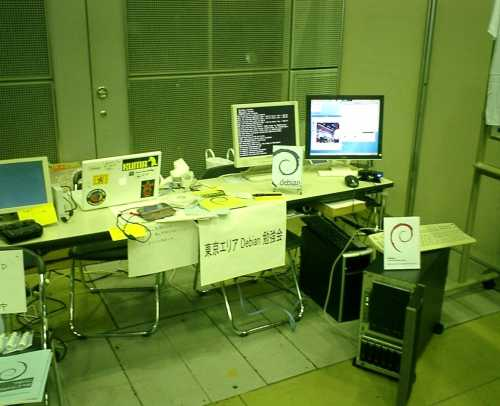
\includegraphics[width=0.45\hsize]{image200710/booth.jpg}
  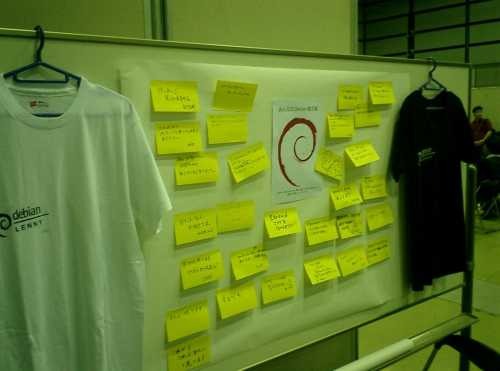
\includegraphics[width=0.45\hsize]{image200710/whiteboard.jpg}
 \end{center}
 \caption{ブースの様子}
 \label{fig:oscfalldebbooth2}
 \end{figure}
\end{frame}

\begin{frame}{OSCでのサーバ機器試験サマリー}
 \begin{itemize}
  \item OSC Tokyo Fall で展示した
  \item ついでにサーバ機器を借りてDebianをいれていろいろといじってみた
  \item できたこと
	\begin{itemize}
	 \item etch のインストールと稼働テスト
	\end{itemize}
  \item できなかったこと
	\begin{itemize}
	 \item iLO, IPMI などのサーバ的な機能をいじること
	\end{itemize}
 \end{itemize}
\end{frame}

\section{ML350G5}
\begin{frame}{ML350G5 Debian etch 動作確認}

 \begin{minipage}[t]{0.45\hsize}
\begin{itemize}
 \item Intel Xeon CPU 搭載
 \item 300GB SAS ディスク6本搭載
\end{itemize}
 \end{minipage}
 \begin{minipage}[t]{0.45\hsize}
  \begin{itemize}
   \item 機動時に F8 をおしてRAIDの設定
   \item i386 でも amd64 でもインストール可能
   \item グラフィックカードは ATI、debconf が自動認識
  \end{itemize}
 \end{minipage}
\end{frame}

\section{ML110G4}
\begin{frame}{ML110G4 Debian etch 動作確認}

 \begin{minipage}[t]{0.45\hsize}
\begin{itemize}
 \item Intel Celeron CPU 搭載
 \item SATA接続ディスク搭載モデル
\end{itemize}
 \end{minipage}
 \begin{minipage}[t]{0.45\hsize}
  \begin{itemize}
   \item i386 でインストール実施。
   \item グラフィックカードは MGA、自動で認識できない。また、ビデオメモ
	 リが少ない。24ビットのままだと 640x480 になるため、色を16bit に
	 減らして 1024x768x16 で稼働させた。
  \end{itemize}
 \end{minipage}
\end{frame}

\section{Eyetoy}
\begin{frame}[containsverbatim]{Eyetoy}
 \subsection{USB webcam の認識}

 PlayStation2 用USBカメラ EyeToy

 ov51x-jpeg が必要のため、バックポート

   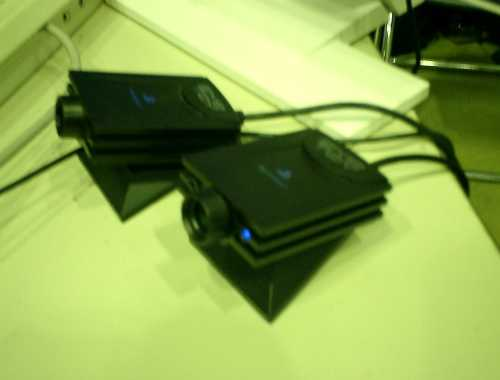
\includegraphics[width=0.5\hsize]{image200710/eyetoy.jpg}

\begin{commandline}
debian:/home/hoge/ov51x-jpeg# apt-get install linux-headers-2.6.18-5-amd64 \
 linux-kbuild-2.6.18 linux-source-2.6.18
debian:/home/hoge/ov51x-jpeg# make make -C
debian:/home/hoge/ov51x-jpeg# insmod v4l1-compat.ko
debian:/home/hoge/ov51x-jpeg# insmod v4l2-common.ko
debian:/home/hoge/ov51x-jpeg# insmod videodev.ko
debian:/home/hoge/ov51x-jpeg# insmod ov51x-jpeg.ko
\end{commandline}

\end{frame}

\section{最近のイベント}
\begin{frame}{最近のイベント}
\begin{itemize}
 \item 11月17日 OSC 沖縄
 \item 11月17-24日 CodeFest
 \item 11月19日 カーネル読書会
 \item 11月25日 仮想化友の会(場所未定)
 \item 12月15日 Debian勉強会
\end{itemize}
\end{frame}

\end{document}
